%!TEX root = ../main.tex
%
% モンテカルロ法によるシミュレーション
%


\section{モンテカルロ法によるシミュレーション}

\subsection{モンテカルロ法とは }

厳密に(解析的に)解けない問題の答えを求めるために、モンテカルロ法と呼ばれ 
る、確率論を利用した数値解析を行なうことがあります。これは、計算機物理学と呼 
ばれる分野で使われる解析方法です。計算機物理学は、理論物理学、実験物理学と並 
ぶ物理学の重要な分野の一つです。

この実験では、既に分かっている面積を測定することにモンテカルロ法を用い、そ 
の結果を使って円周率$\pi$の値を求めてみましょう。 

\subsection{モンテカルロ法による円周率の計算}
\label{MC:keisan}

下図の斜線の部分(扇形)の面積を、モンテカルロ法により求めてみましょう。
\begin{center}
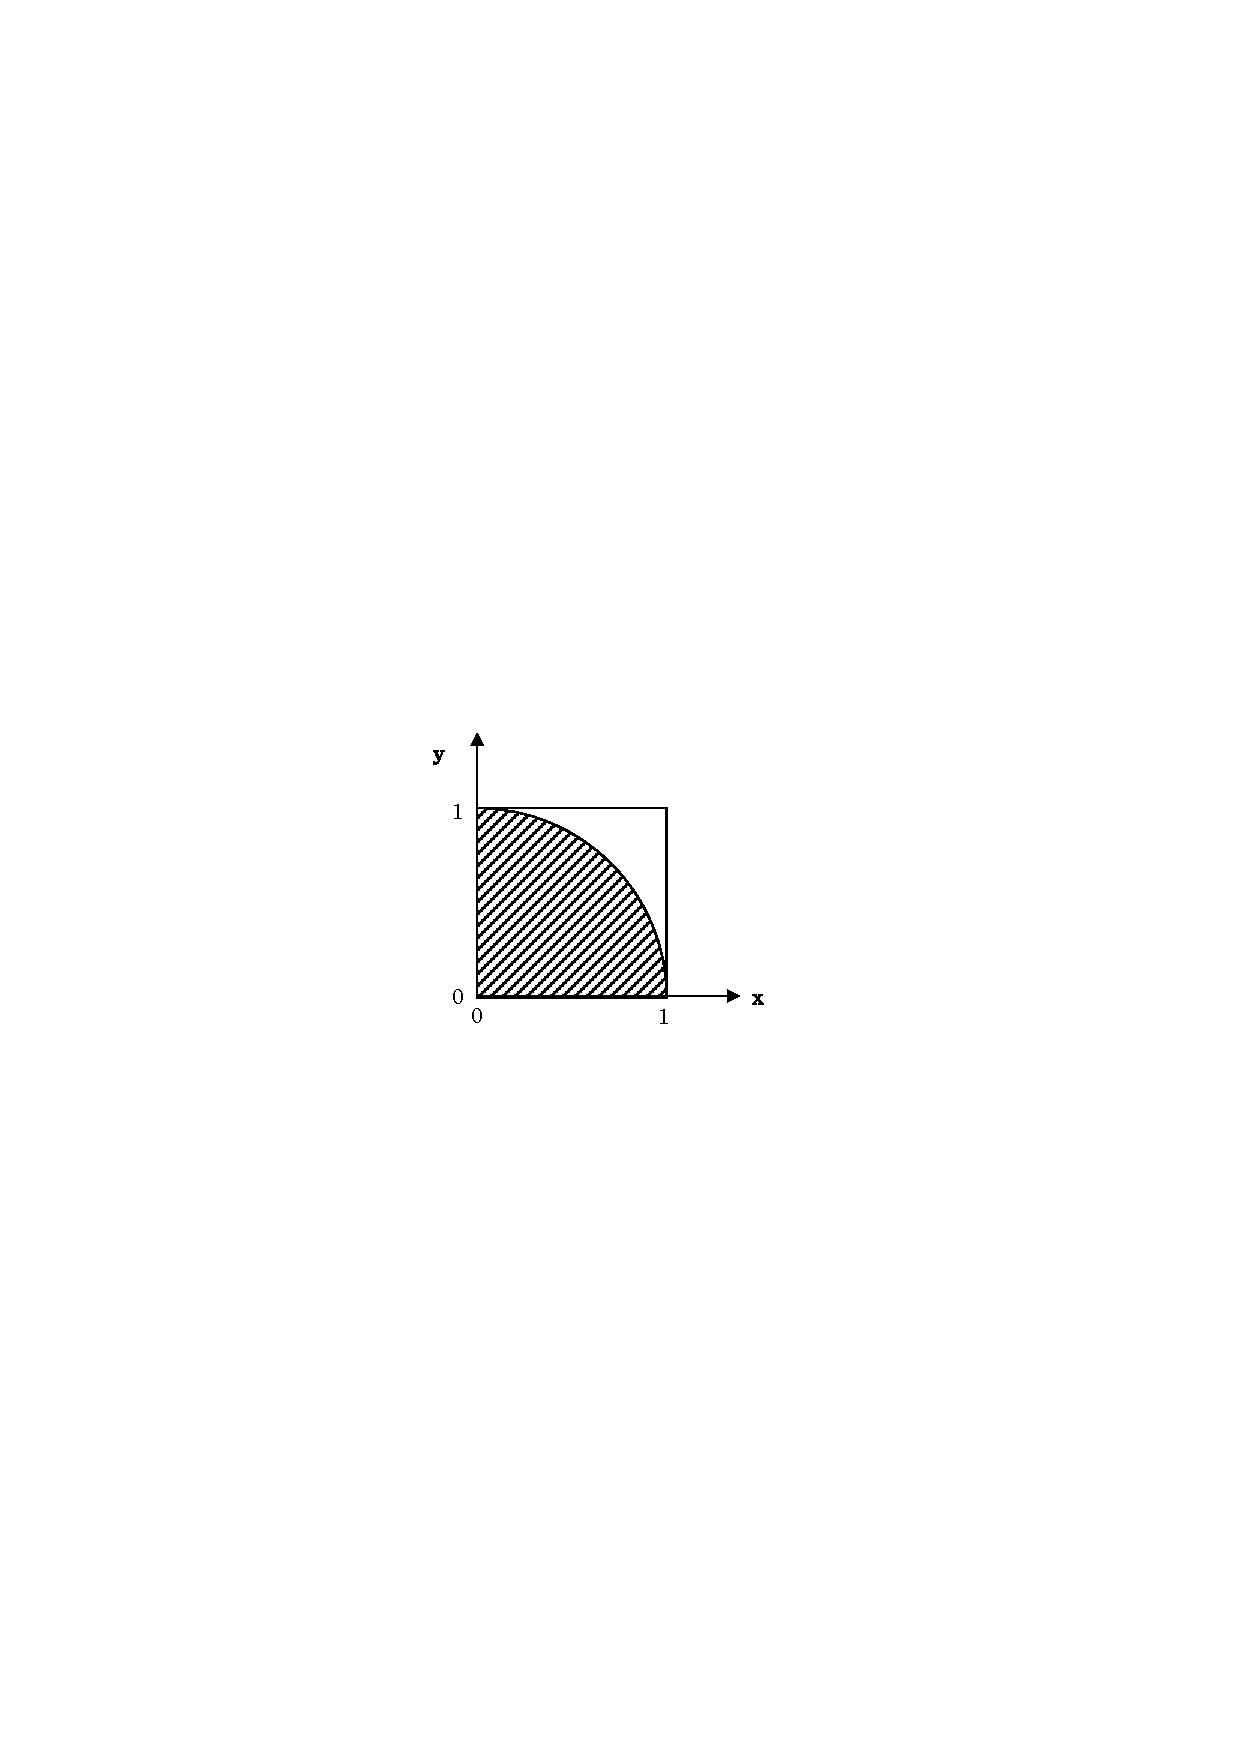
\includegraphics[bb=193 342 378 499]{08_MonteCarlo/montecarlo1.pdf}
\end{center}
そのためには、上のような$0\leq x \leq 1$、$0\leq y \leq 1$の正方形(面積1)の中に、ランダ 
ムに多数の点をプロットして、全体の点の数に対し、斜線部分にプロットした点の数 
が幾つあるかを数えることで、斜線部分の面積を求めることができます。

ランダムに点をプロットするためには、乱数を使います。乱数とは、何の規則もな 
くばらばらに分布している数のことです。例えば、特殊なサイコロを振って、0から 
0.99までの間の数を二回出し、それを$(x,y)$座標とみなして点をプロットしていき 
ます。すると、確率論では、点を多くプロットすれば、単位面積あたりの点の数は一 
定の数に近づくことになります。

つまり、近似的に、
\begin{center}
\fbox{$\displaystyle{\frac{斜線部分の面積}{正方形の面積} \approx \frac{斜線部分の点の総数}{正方形内の点の総数}}$}
\end{center}
という式が成り立つことになります。この式から、斜線部分の面積を求めることがで 
きます。

また、円の面積を求める式を使うと、図の斜線部分の面積は、半径1の円の面積の 
4分の1なので、$\pi/4$になるということが分かります。よって、 
\[ 
「斜線部分の面積」= \pi/4
\]
より、円周率:$\pi$を求めることができます。これを実際に実験で求めてみましょう。

\bigskip


\begin{wrapfigure}[7]{r}{5cm}
\vspace*{-0.8cm}
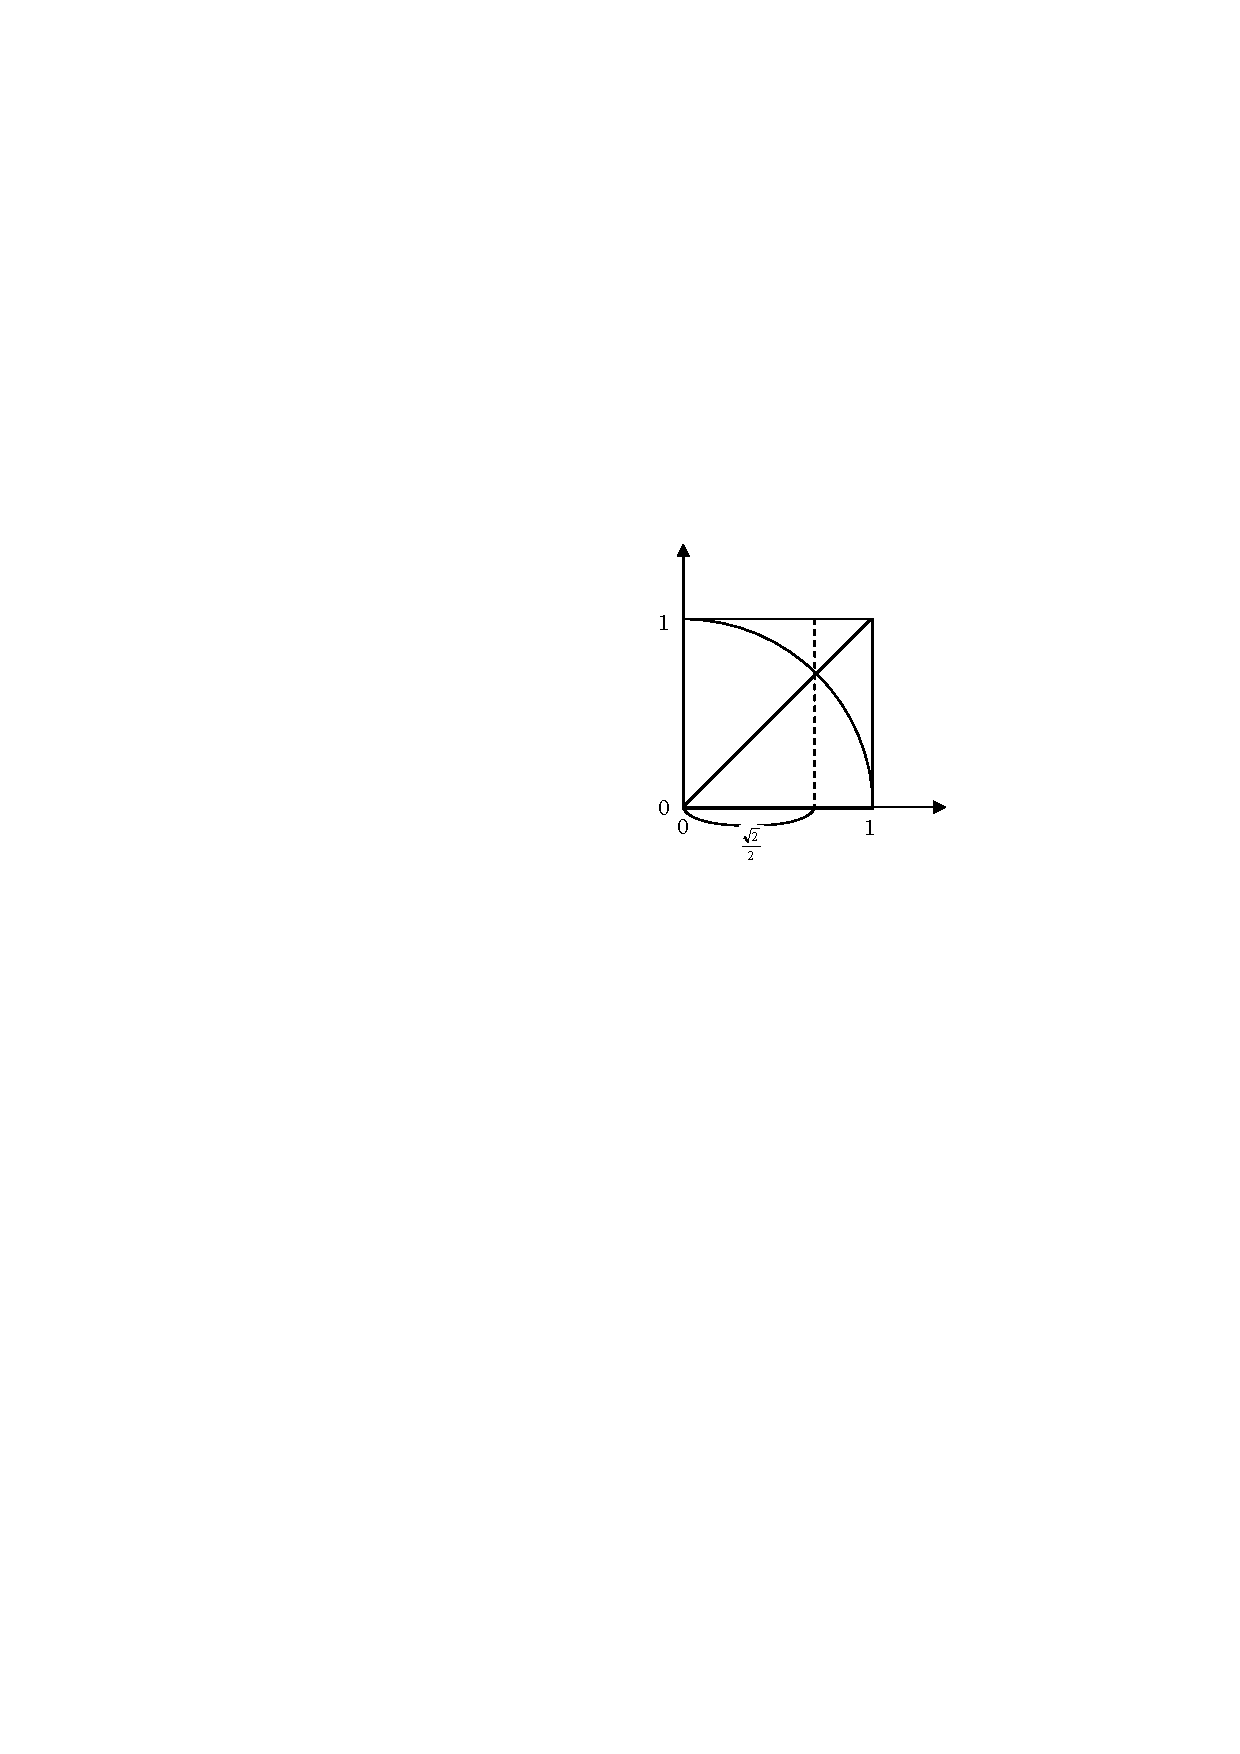
\includegraphics[bb=303 425 461 582]{08_MonteCarlo/montecarlo2.pdf}
\end{wrapfigure}

\paragraph{考察}
\ref{MC:keisan}の実験の結果を利用して、$\sqrt{2}$の値を求めることができます。どのよう
にすれば$\sqrt{2}$の値が求められるかを考えてみましょう。

\bigskip

\hspace*{-\parindent}<考察のヒント>

右の図のように、正方形に対角
線を描き、対角線と円の弧の交点
から$x$軸上に垂線を下ろすと、原
点から垂線の足までの距離は、$\frac{\sqrt{2}}{2}$
になります。 



\bigskip

\begin{itembox}[l]{\bf コラム:乱数の利用}
乱数の利用は、農事試験など大規模で実験がやりにくい実験計画において、偶然のばらつ
きを消すように統計的処理をするために、イギリス人フィッシャーが考案したと言われ
ている。今日では、統計的品質管理の抜き取り検査や、シミュレーション実験に広く使
われている。乱数は暗号作成と解読などにも利用されているので、推理小説やスパイ事
件などでなじみのある人もいるだろう。
\end{itembox}

\newpage

\jikken

\begin{itemsquarebox}[c]{\bf 実験用具}
方眼紙、乱数サイ、(プログラミングによる円周率の計算を行なう場合は、プ 
ログラミング言語の扱えるパソコン)
\end{itemsquarebox}

\bigskip

\subjikken{乱数サイを用いた円周率の計算}

「乱数サイ」とは、20面体のサイコロの各面に、0から9までの数字がそれぞれ 
2面ずつ配置されたものです。この実験では、正方形の中にランダムに点を打つ 
ために、この乱数サイを使用します。

\begin{enumerate}

\item 方眼紙に、正方形を記入し、その中に正方形の1辺を半径とする円の1/4にあた 
る扇形を描いておきます。(正方形の縦と横に0〜100までの座標をつけます。 )

\item 色の違う2個の乱数サイを1組とし、$x$座標用、$y$座標用にそれぞれ1組ずつ用 
意します。これを左右の手に1組ずつ持って振り、2桁の乱数を発生させます。

\item 方眼紙上で、乱数サイで得られた100個の点の座標を25個ずつ区別しながら記入します。

\item 上の\maru{2}〜\maru{3}の操作を100回繰り返し、扇形の中に入っている印の数から、円周率 
の値を求めます。

\end{enumerate}

\subjikken{プログラミングによる、乱数を用いた円周率の計算}

乱数サイを使って行なったことを、計算機で行なってみましょう。計算機を使う
と、乱数サイで行なった操作を短時間で実行することができるため、100回以上
サイコロを振った場合の円周率を求めることができます。

\begin{enumerate}

\item Processingというプログラミング言語を実行するアプリケーションを起動し、プログラム例にあるプログラムを入力します。\\
※  ProcessingはWindows用とMac用が{\tt http://www.processing.org/}からダウンロードできます。

\item Nという変数の値がサイコロを振る回数です。サイコロを振る回数を決定しプログラムを実行します。(10,000,000回以下)

\item $1/4$の円内に入った点は青色、入らなかった点は赤色で表示されます。

\item さいころを振る回数を変えて何度かプログラムを実行してみましょう。点の数が多くなると円の形がはっきりとしてきます。(一回の計算にかかる時間を確認してから、回数を増やすようにしましょう。)

\end{enumerate}

サイコロを振る回数を100回から開始して、1,000回、1万回…と増やしていき、得 
られた円周率の値を記録しましょう。

\bigskip

\underline{\bf Processingを用いた円周率の計算のプログラム例:}



\begin{screen}
\begin{verbatim}
size(500,500); //画面のサイズ

int N = 100; //繰り返しの数(点の総数)
int c = 0;   //円内の点の数を数えるカウンタ

for (int i=0; i<N; i++){     //N回繰り返す
  float x = random(0.0,1.0); //0から1までの乱数(x)
  float y = random(0.0,1.0); //0から1までの乱数(y)
  
  if( x*x+y*y < 1.0){       //もし円の中なら
    c++;                    //カウンタを1つ増やす
    stroke(color(0,0,255)); //ペンの色を青にする
    point(x*500, y*500);    //画面に点を打つ
  }else{                    //円の外ならカウンタは増やさない
    stroke(color(255,0,0)); //ペンの色を赤にする
    point(x*500, y*500);    //画面に点を打つ
  }
}

float pi = float(c)/float(N)*4.0; //(円内の点数)/(点の総数)x4が円周率
print("pi=" + pi); //円周率の値を画面に出力する
\end{verbatim}
\end{screen}
